%!TEX root = main.tex

\chapter{Preliminares}
\label{cap:preliminares-v2}
A notação que usamos na tese é a comumente adotada na maioria dos textos de teoria dos grafos, combinatória poliédrica e otimização combinatória, que são as  disciplinas que permeiam este trabalho. Apresentamos apenas alguns conceitos básicos para estabelecer a terminologia, e em cada seção sugerimos ao leitor a consulta de outros textos, caso alguns conceitos não estejam definidos aqui.

%% Para conceitos em otimização combinatória, incluindo tópicos como \emph{branch-and-bound} e \emph{branch-and-price}, o leitor poderá utilizar as referências~\cite{Wolsey1998,BarnhartJNSV1998,NemhauserW1999,DesrosiersL2005,MorrisonJSS2016}.

 % Para obter informações sobre algoritmos de aproximação, o leitor poderá utilizar como referência Ausiello et al~\cite{AusielloPMGCK1999}.  

% Para as definições das classes específicas de grafos, o leitor poderá utilizar as referências \cite{BrandstadtLS1999,GrossYZ2013,BrandstadtDLL2004}.

\section{Conceitos básicos sobre grafos}

Um \emph{grafo} é um par ordenado $(V,E)$, onde $V$ é um conjunto de elementos chamados \emph{vértices}, e $E$ é um conjunto de pares não ordenados de elementos distintos de $V$, chamados \emph{arestas}. Se $G$ é o nome de um grafo definido por um par $(V,E)$, então escrevemos $G=(V,E)$. Algumas vezes, referimos simplesmente a um grafo~$G$, e usamos a notação $V(G)$ e $E(G)$, respectivamente, para denotar o seu conjunto de vértices e de arestas. Muitas vezes, uma aresta $e = \{u,v\}$ é denotada por $uv$ (ou $vu$). Se $e=uv$, os vértices $u$ e $v$ são chamados \emph{extremos} da aresta~$e$. Em geral, mesmo não estando explícito, denotamos por $n$ o número de vértices do grafo em consideração.

Um \emph{subgrafo} $G'$ de $G=(V,E)$ é um grafo, onde
$V(G')\subseteq V$ e $E(G')\subseteq E$. Usamos a notação
$G'\subseteq G$ para indicar que $G'$ é um subgrafo de $G$. Se
$G'\subseteq G$ e $V(G')=V$, então dizemos que $G'$ é um subgrafo
\emph{gerador} de $G$.  Para $W\subseteq V$, dizemos que $G'$ é um
subgrafo \emph{induzido} por $W$, se $V(G')=W$ e para cada par
$u,v \in W$, temos que $uv \in E(G')$ se e só se $uv\in E$. Neste
caso, escrevemos $G' = G[W]$. Para $F \subseteq E$, dizemos que $G'$ é
um subgrafo \emph{induzido} por $F$, e escrevemos $G' = G[F]$, se
$E(G')=F$ e $V(G')$ é o conjunto dos vértices de $V(G)$ que são
extremos das arestas em $F$.

% Um conjunto $\mathcal{P} = \{P_1, P_2, ..., P_i\}$ de subconjuntos de um conjunto $P$ é chamado de \emph{partição} de $P$ se $\bigcup_{1..i}P_i = P$ e, para $1 \le x < y \le i$, $P_x \cap P_y = \emptyset$.

Num grafo $G=(V,E)$, dois vértices $u,v$ são \emph{adjacentes} ou \emph{vizinhos} em $G$ se $uv \in E$. O conjunto dos vizinhos de um vértice $u$ é o conjunto 
 $N_{u}(G)= \{v \in V\; |\; uv \in E\}$. O \emph{grau} de um vértice $v \in V$ é a quantidade de arestas adjacentes a $v$ em $G$.

 Seja $P = (v_1,a_1, v_2,a_2, \ldots, a_{k-1},v_k)$, com $k\ge 1$, uma sequência alternada de vértices ($v_i$) e arestas ($a_i$) de $G$.  Esta sequência é chamada de \emph{caminho} se os vértices são dois a dois distintos e para $1 \le i < k$, $a_i = v_{i}v_{i+1}$. O \emph{comprimento} de $P$ é $k$, a quantidade de suas arestas. Como um caminho fica bem determinado pela sequência de seus vértices, comumente denotamos um caminho apenas pela sequência de seus vértices: no caso do caminho $P$, este se simplificaria para $(v_1,v_2,\ldots,v_k)$. Dizemos que $P$ é um caminho de $v_1$ a $v_k$ (ou entre $v_1$ e $v_k$). A \emph{distância} entre dois vértices $u$ e $v$ num grafo $G$, denotada por $\dist_{G}(u,v)$,  é definida como o comprimento de um caminho de menor comprimento entre $u$ e $v$ em~$G$.

Se $P = (v_1,v_2,\ldots,v_k)$ é um caminho, e existe em $G$ a aresta $v_kv_1$, então a sequência $(v_1,v_2,\ldots,v_k,v_1)$ define um \emph{circuito} em $G$.
%% ????? Muitas vezes, basta indicamos apenas os vértices distintos do circuito. 

Dizemos que $G$ é um grafo \emph{conexo} se em $G$ existem caminhos entre todos os seus pares de vértices.  Um conjunto de vértices $I$  de um grafo $G$ é \emph{independente} se para cada $u,v \in I$, tem-se que $uv \notin E$.

Definimos a seguir algumas operações que são comumente realizadas em
grafos: \emph{remoção de vértices}, \emph{remoção de arestas} e
\emph{contração de arestas}. A \emph{remoção de um vértice} $u$ de um
grafo $G$ resulta em um subgrafo $G'=(V \setminus \{u\},E')$, onde $E'
= E \setminus \{uv\in E \; | \; v\in N_{u}(G) \}$. A \emph{remoção de uma aresta} $e$ de $G$ resulta em um subgrafo $G'=(V,E \setminus \{e\})$. A \emph{contração de uma aresta} $uv$ de $G$ resulta em um grafo $G'$ que se obtém de $G$ removendo-se os vértices $u$ e $v$ e acrescentando um novo vértice, digamos $w$, e fazendo-o adjacente aos vértices   
de ($N_{u}(G) \cup N_{v}(G))\setminus\{u,v\}$. Neste caso, $|V(G')| = |V|-1$.


% %% resulta em um grafo $G'(V \setminus \{u,v\} \cup \{m_{u,v}\},E')$,
% %% onde $E' = E \setminus \{xy \in E\; |\; x = u \text{ ou } x = v\} \cup \{xy \in E\; |\; x = u\}$ corresponde a remover tal aresta e
% juntar os vértices $u$ e $v$ num vértice só, e os vizinhos em $G$ deste
% novo vértice serão os vizinhos de $u$ e $v$ em $G$ (excluindo a aresta $uv$). 
% %% substituir os vértices $u$ e $v$ por um
% %% único vértice e pelas arestas incidentes somente em $u$ ou somente em $v$.

Um conjunto $C \subseteq V$ é uma \emph{clique} de $G$ se os vértices de $C$ são dois a dois adjacentes. Algumas vezes, também chamamos de clique o subgrafo de $G$ induzido por $C$.

Um \emph{grafo direcionado} ou \emph{digrafo} é um par ordenado $(V,A)$, onde $V$ é um conjunto de elementos chamados vértices, e $A$ é um conjunto de pares ordenados de vértices distintos de $V$, chamado \emph{arcos}. Também representamos um arco $a = (u,v) \in A$ simplesmente por $uv$ (aqui a ordem dos vértices é importante); e dizemos que o vértice $u$ é o de \emph{origem} e o vértice $v$ é o de \emph{destino}. Também usamos a notação $V(D)$ e $A(D)$, respectivamente, para
denotar o conjunto de vértices e de arcos de $D$.

Para consultar outros conceitos da teoria dos grafos, sugerimos Bondy e Murty~\cite{BondyM2008}, Bollobás~\cite{Bollobas1998} ou Diestel~\cite{Diestel2017}.

\subsection{Algumas classes de grafos}
A seguir, definiremos algumas classes especiais de grafos, que serão mencionados neste trabalho. 

O \emph{complemento} de um grafo $G$ é um grafo $H$ sobre o mesmo conjunto de vértices tal que dois vértices distintos de $H$ são adjacentes se e só se não são adjacentes em $G$.

Um grafo $G$ é \emph{bipartido} se $V$ admite uma bipartição $X\cup Y$ tal que todas as arestas de $G$ têm um extremo em $X$ e outro em $Y$. Neste caso, para explicitar a bipartição, escrevemos que $G=(X\cup Y, E)$. 

Um \emph{cografo} é um grafo que consiste de um único vértice, ou é a união disjunta de dois cografos, ou é o complemento de um cografo.
Um grafo \emph{split} é um grafo que pode ser particionado em uma clique e um
conjunto independente.
%
Um grafo \emph{intervalo} é um grafo cujos vértices estão em correspondência um-a-um com uma coleção finita de intervalos da reta real, ou seja, cada vértice corresponde a um intervalo; e dois vértices são adjacentes se os correspondentes intervalos têm intersecção não vazia.

Um \emph{grafo de permutação} é um grafo cujos vértices representam os elementos de uma permutação, e cujas arestas representam pares de elementos que são invertidos pela permutação. 


% Sejam $\mathcal{L}_1$ e $\mathcal{L}_2$ duas linhas paralelas e sejam
% $P = \{1,2,\dots,n\}$ um conjunto de pontos sobre $\mathcal{L}_1$ e
% $\mathcal{L}_2$. Para cada $i \in P$, seja $L_i$ a linha que liga $i$ em
% $\mathcal{L}_1$ a $i$ em $\mathcal{L}_2$. 
% Seja $G=(P, E_{\mathcal{L}})$ onde $ij \in E_{\mathcal{L}}$ se $L_i$ e $L_j$ se
% cruzam. O grafo $G=(P, E_{\mathcal{L}})$ é chamado de grafo \emph{permutação}.

Um grafo é \emph{planar} se pode ser desenhado no plano sem que haja intersecção de suas arestas, exceto em seus extremos.  Um grafo planar é \emph{exoplanar} se pode ser desenhado no plano de modo que todos os seus vértices pertençam à  fronteira da face externa.

Um grafo bipartido $G=(X \cup Y, E)$ é \emph{convexo} sobre $X$ se
existe uma ordenação de $X$ tal que para cada $y \in Y$, os vértices
adjacentes a $y$ são consecutivos na ordenação de $X$.

Um grafo $G=(V,E)$ é de \emph{comparabilidade} se admite que suas arestas possam ser orientadas de modo a produzir um digrafo $D=(V,A)$ que é uma orientação transitiva,  ou seja, sempre que  $xy\in A$ e $yz \in A$, então $xz \in A$. Um grafo é de \emph{cocomparabilidade} se seu complemento é um grafo de comparabilidade.

Um vértice $v$ num grafo~$G$ é \emph{simplicial} se os vizinhos de~$v$ formam uma clique em $G$. Um grafo~$G$ é \emph{$1$-split} se ao removermos todos os vértices simpliciais de $G$ resta somente uma clique.

Um grafo $G$ é \emph{cordal} se para todo circuito de comprimento pelo menos quatro tem uma corda, que é uma aresta que 
não faz parte do circuito mas conecta dois vértices do circuito. Para um circuito de comprimento par, uma corda neste circuito é ímpar se os dois vértices adjacentes pela corda são separados no circuito por uma distância ímpar. Um grafo é \emph{fortemente cordal} se é cordal e para cada circuito de comprimento par e maior ou igual a seis  existe uma corda ímpar.

Chamamos de \emph{hipercubo} um grafo cujos vértices e cujas arestas correspondem, respectivamente, aos vértices e às arestas de um hipercubo.

Um grafo $H$ é \emph{menor} de um grafo $G$ se $H$ pode ser obtido a partir de
$G$ por meio da remoção de vértices, remoção de arestas ou contração de arestas.

Para ver definições de outras classes de grafos, ou relações entre essas classes, o leitor poderá consultar as referências \cite{BrandstadtLS1999,BrandstadtDLL2004,GrossYZ2013}.


\section{Conceitos básicos sobre poliedros}
\label{sec:poliedros}

Sejam $x_1, x_2, ..., x_m$ vetores em $\espacoRn$. Dizemos que um vetor $x$
é uma \emph{combinação linear} de $x_1, x_2, ..., x_m$, se 
$x = \sum_{i=1}^{m}\lambda_i x_i$, onde $\lambda_1, \lambda_2, ..., \lambda_m \in \espacoR$. Se, adicionalmente, temos que  $\sum_{i=1}^{m} \lambda_i = 1$, então dizemos que $x$ é uma \emph{combinação afim} de $x_1, x_2, ..., x_m$. Uma combinação afim como a acima, com $\lambda_1, \lambda_2, ..., \lambda_m \in \espacoRpos$, é chamada de \emph{combinação convexa} de $x_1, x_2, ..., x_m$.

% % , se $x = \sum_{i=1}^{m}\lambda_i x_i$, onde $\lambda_1, \lambda_2, ..., \lambda_m \in \espacoRpos$, e $\sum_{i=1}^{m} \lambda_i = 1$.

% , então um vetor $x = \sum_{i=1}^{m}\lambda_i x_i$ é chamado de \emph{combinação convexa} dos vetores $x_1, x_2, ..., x_m$.  Um vetor $x \in \espacoRn$ é uma \emph{combinação afim} dos vetores $y$ e $z$ se existe $\lambda \in \espacoR$ tal que $x = \lambda y + (1 - \lambda) z$. 

Dizemos que vetores $x_1, x_2, ..., x_m \in \espacoRn$ são
\emph{linearmente independentes} se o sistema $\sum_{i = 1}^{m}
\lambda_i x_i = \vec{0}$, $\lambda_i \in \espacoR$, tem como única
solução $\lambda_i = 0$ para $i = 1,\ldots,m$. Dizemos que vetores
$x_1, x_2, ..., x_m \in \espacoRn$ são \emph{afim-independentes} se o
sistema $\sum_{i = 1}^{m} \lambda_i x_i = \vec{0}$, $\lambda_i \in
\espacoR$, $\sum_{i = i}^{m} \lambda_i = 0$ tem como única solução
$\lambda_i = 0$ para $i = 1, \ldots,m$.  O \emph{fecho convexo} de um
conjunto $S \in \espacoRn$ é o conjunto dos vetores em $\espacoRn$ que
podem ser escritos como combinação convexa dos vetores em $S$.
 O \emph{fecho inteiro} de um
conjunto $S \in \espacoRn$ é o conjunto dos vetores em $\espacoRn$ que
podem ser escritos como combinação convexa dos vetores inteiros em $S$.
%% De maneira análoga podemos definir um
%% \emph{fecho afim} de um conjunto $S \in \espacoRn$.

Um \emph{poliedro} $P$ em $\espacoRn$ é um conjunto da forma $\{x \in \espacoRn \; | \; Ax \le b\}$, para alguma matrix $A \in \espacoRmn$ e para algum vetor $b \in \espacoRm$. O poliedro $P$ é chamado de \emph{politopo} se $P$ é o fecho convexo de um conjunto finito de pontos.  A \emph{dimensão} de $P$ é o número máximo de vetores afim-independentes em $P$ menos um.
%% fecho afim de $P$. Representamos a dimensão de $P$ por $dim(P)$.

Dado um poliedro da forma $Q = \{(u,x) \in \espacoRp \times
  \espacoRq: Au + Bx \le b\}$, para matrizes $A \in \espacoRmp$ e $B \in
  \espacoRmq$ e para algum
  vetor $b \in \espacoRm$, a \emph{projeção} de $Q$ no espaço da variável $x$
  (ou seja, no espaço $\espacoRq$) é definida como 
 $$Proj_x(Q) = \{x \in \espacoRq\; | \; \exists u \in \espacoRp \text{
   tal que } (u,x) \in Q \}.$$
 

 Para definições e resultados básicos sobre combinatória poliédrica, o leitor pode consultar~\cite{FerreiraW1996}; e sobre projeções, 
 indicamos~\cite{Balas2005}.


\section{Otimização combinatória}
\label{sec:otimizacao}

\emph{Problemas de Otimização Combinatória Linear} (POC) podem ser definidos
por meio de
de uma tripla $(E, w, \Scal)$, onde
%% $\Ical$ representa um conjunto de instâncias, 
%% onde
$E$ é um conjunto finito e não vazio, $w: E \to \espacoRpos$ é
uma função peso, e $\Scal$ representa soluções viáveis formadas por
subconjuntos de $E$. O objetivo é encontrar uma solução $S \in \Scal$ que
maximiza ou minimiza o valor da solução, dado por $f(S) = \sum_{e \in S} w_e$.
A função $f(S)$ é chamada de \emph{função objetivo}.
Neste trabalho, para uma função objetivo
  $w: E \to \espacoRpos$
  e para $e \in E$, usamos a  notação $w_e$ em vez de $w(e)$.
Vamos assumir que estamos trabalhando com problemas de minimização.
Observe que estamos apenas considerando funções objetivo lineares,
visto que os problemas de otimização ao longo desta tese terão apenas
este tipo de função objetivo. Isto não quer dizer que todos os problemas
de otimização terão esta classe específica de função objetivo.

Para cada POC definido pela tripla $(E, w, \Scal)$, podemos associar um poliedro. Para definir um tal poliedro, precisamos definir alguns conceitos antes. Para um espaço vetorial real $|E|$-dimensional $\espacoEDef$, seja $x \in \espacoEDef$ um vetor cujos componentes são indexados pelos elementos de $E$. Para cada solução $S \in \Scal$, consideremos o \emph{vetor de incidência} $\incid^{S} = (\incid^{E}_{e})_{e \in E}$, definido como

  \begin{align*}
    &\incid^{S}_{e}=
      \begin{cases}
        1,& \text{se $e \in S,$}\\
        0,& \text{caso contrário.}
      \end{cases}
  \end{align*}

  Podemos então associar um poliedro $P \subseteq \espacoEDef$ à tripla
  $(E, w, \Scal)$ como sendo o fecho convexo dos vetores de incidência
  das soluções em $\Scal$, isto é
\begin{equation*}
\begin{split}
P :=  \text{conv}\{\incid^{S} \in \espacoXDef\; |\; S \in \Scal\}. 
\end{split}
\end{equation*}
Dessa forma, o POC considerado pode ser definido como
$\min \; \{w^{\intercal}x \; |\; x \in P\}$.  O conjunto dos vértices
de $P$ corresponde ao conjunto dos vetores de incidência das soluções
$S \in \Scal$ (veja~\cite{FerreiraW1996}). Como $P$ é um politopo,
então sabemos que $P$ pode ser descrito por meio de um sistema de
inequações lineares. Desta forma, podemos modelar um POC como um
problema de \emph{Programação Linear} (PL). Ou seja, é possível
modelar todo POC como um PL 0/1. Reciprocamente, como mencionado
em~\cite{FerreiraW1996}, todo PL 0/1 pode ser formulado como um
POC. De fato, dado um PL 0/1 da forma
$\min\; \{w^{\intercal}x \; |\; Ax \le b,\; x \in \{0,1\}^n \}$, onde
$A \in \espacoRmn$ e $b \in \espacoRm$, podemos formular este PL como
um POC definido sobre $(E, w, \Scal)$, onde $E := \{1,2,...,n\}$ e
$\Scal := \{S \subseteq E\; |\; A\incid^{S} \le b\}$.

Considere o programa linear
%% $z = \min\{w^{\intercal}x \; |\; Ax \le b,\; x \in \espacoRn \}$,
$z = \min\{w^{\intercal}x \; |\; x \in P\}$,
onde $P = \{x \in \espacoNBinary \; | \; Ax \le b\}$,
$A \in \espacoRmn$ e $b \in \espacoRm$.
%% Vamos chamar este PL de $(P)$. 
Seja $a_ix \le b_i$, $1 \le i \le m$, a $i$-ésima restrição do conjunto de restrições de $P$.  
Um vetor $x \in P$ %que satisfaça $Ax \le B$
é chamado de
\emph{solução viável} de $Q$, e o valor de $z$ é chamado de
\emph{valor ótimo} de $Q$. Uma solução viável $x^*$ para a qual o valor ótimo é atingido é chamada de
\emph{solução ótima}. 
%%%%%%%%%%%%%%%%%%%%%%
O \emph{suporte} de um vetor~$x$ é o conjunto dos índices~$i$ tais que
$x_i \ne 0$. Dizemos que uma solução viável~$x$ tem \emph{suporte
  minimal} se não existe outro vetor viável~$x'$ cujo suporte esteja
contido propriamente no suporte do vetor~$x$. 
Para um vetor $x' \in \espacoNBinary$, uma restrição 
$a_ix \le b_i$ de $P$  é dita \emph{ativa} em $x'$ se $a_ix' = b_i$. 
% Uma solução \emph{básica} viável $x \in P$ é aquela que satisfaz $n$ restrições
% linearmente independentes. 

%%%%%%
%% Seja $Q$ um problema, formulado como um programa linear inteiro da forma:
%% $\min  \{x \in \espacoRn \; | \; Ax \le b, \; x \; \hbox{inteiro} \}$,
%% onde  $A \in \espacoRmn$ e $b \in \espacoRm$. Considere o programa linear
%% $P'$  relaxado correspondente, $\min \{x \in \espacoRn \; | \; Ax \le
%%  b\}$. Dado um conjunto de instancias ${\cal {I}}$ do problema~$Q$, o \emph{gap de integralidade}
%% relativo à formulação linear acima é definido como
%% $$ \sup_{I\in {\cal I}} \frac{\opt(I)}{\opt_f(I)},$$
%% onde $\opt(I)$ é o valor da solução ótima (inteira) de $Q$ para a
%% instância~$I$, e $\opt_f(I)$ é o valor da solução ótima do programa
%% linear relaxado $P'$ para a instância~$I$.

% %%%%%%%%%%%%%%%%%%%%%%%%%%%%
%      {\color{red}
%        Para um problema de minimização, o \emph{intervalo}
%        (\emph{gap}) de integralidade consiste na diferença entre a melhor
%      (menor) 
%      solução inteira e a melhor (maior) cota inferior para a função objetivo.
%      No nosso caso, expressaremos essa diferença de maneira relativa, mais
%      especificamente:
%      \begin{align*}
%        ((MelhorSolInteira - MelhorCotaInf) / MelhorSolInteira) * 100,
%      \end{align*}
%      onde \emph{MelhorSolInteira} corresponde à melhor solução inteira e
%      \emph{MelhorCotaInf} corresponde à melhor cota inferior para a função
%      objetivo.
%      }
     
\subsection{Problema da separação}
Um resultado extremamente importante na área de otimização diz respeito à equivalência entre problema de otimização e \emph{problema da separação}.  Este assunto e outros correlatos foram seminalmente tratados por Grötschel, Lovász e Schrijver~\cite{GrotschelLS1988}.  No problema da separação, dado um poliedro e um ponto no mesmo espaço vetorial,
%% (possível) solução,
queremos saber se existe uma inequação violada pelo ponto.  Em outras palavras, desejamos saber se o ponto pertence ao poliedro ou obter um certificado (da não pertinência) que corresponda a uma inequação violada.

Mesmo quando um poliedro possui um número exponencial de inequações, é possível otimizar uma função objetivo neste poliedro, fazendo algumas restrições na entrada do problema. Apesar de não existir um algoritmo fortemente polinomial (ou seja, que não dependa da representação da entrada) para problemas de programação linear, usando o \emph{método elipsóide} e fazendo algumas restrições na entrada,  é possível resolver em tempo polinomial problemas de otimização desde que o problema de separação seja resolvido em tempo polinomial (veja Teorema 3.13 em~\cite{NemhauserW1999}).

\subsection{\emph{Branch-and-bound}}
\label{sec:branch_and_bound}
O método de \emph{branch-and-bound} (B\&B) é utilizado para resolver (de maneira exata) problemas difíceis de otimização.
%% Nós utilizaremos como base o trabalho de Morrison et
%% al~\cite{MorrisonJSS2016} para descrever este \emph{framework}.
Em decorrência dos problemas abordados nesta tese, vamos restringir as definições aos problemas de otimização combinatória linear (POC). Como definido na Seção~\ref{sec:otimizacao}, um POC é definido por uma tripla $(E, w, \Scal)$, onde $\Scal$ representa soluções viáveis formadas por subconjuntos de $E$, e $w: E \to \espacoRpos$ uma função peso.  O objetivo é encontrar uma solução $S \in \Scal$ que minimiza $f(S) = \sum_{e \in S} w_e$. Como dito anteriormente, a função $f: \Scal \to \espacoRpos$ é denominada de \emph{função objetivo}, enquanto que $\Scal$ é conhecido como \emph{espaço de busca}.

O método de B\&B cria uma árvore de busca de subconjuntos do espaço de busca, sendo que estes subconjuntos também são chamados de \emph{subproblemas}. Inicialmente, o B\&B armazena uma solução viável $x^*$ denominada \emph{solução incumbente}.  O algoritmo possui uma lista dos subproblemas (nós) ainda não analisados e, a cada iteração, ele seleciona (e remove da lista) um destes subproblemas.  Vamos considerar que o subproblema selecionado seja $S \subseteq \Scal$. Se for possível encontrar uma solução viável $x \in S$ tal que $f(x) < f(x^*)$, então atualizamos a solução incumbente com $x$. Caso contrário, se for possível provar que não existe solução em $S$ melhor do que a solução incumbente, então o subproblema $S$ é \emph{podado} (operação também conhecida como \emph{podar por otimalidade}~\cite{Wolsey1998}). Caso nenhum dos casos aconteça, subproblemas $S_1, S_2, ..., S_i \subset S$ são criados, sendo que estes correspondem aos nós filhos de $S$ na árvore de busca, e armazenados na lista dos subproblemas ainda não analisados. Quando não houver mais nós na lista a serem analisados, a solução incumbente corresponderá a uma solução ótima.

Existem três componentes importantes no B\&B: a \emph{estratégia de busca},
a \emph{estratégia de ramificação} e a \emph{estratégia de poda}.
A estratégia de busca é responsável por selecionar na árvore de busca o
próximo nó a ser analisado. Duas estratégias de busca conhecidas
são a busca em largura e a busca em profundidade. Uma terceira abordagem,
conhecida como \emph{buscar o melhor primeiro}, será abordada na
Seção~\ref{sec:befs}. A estratégia de ramificação é responsável por definir
como os subproblemas filhos serão criados a partir do subproblema sendo
analisado. Ela também é responsável por saber qual variável fracionária
será selecionada para fazer a ramificação.
Por fim, a estratégia de poda é responsável pelas regras que
vão definir quais nós não precisam ser analisados e podem
ser descartados. Uma destas estratégias é a utilização de
\emph{geração de colunas}. Quando esta estratégia é utilizada juntamente ao
B\&B, o algoritmo é conhecido como \emph{branch-and-price}.

\subsubsection{\emph{Branch-and-price}}
Na geração de colunas, quando o PL  possui muitas
colunas, a maioria destas é deixada de fora da relaxação deste
modelo para que este possa ser resolvido rapidamente. Uma justificativa
para esta abordagem é que numa solução ótima, a maioria das colunas terá 
suas variáveis com valor zero. A versão reduzida (com menos colunas) da
relaxação do PL é conhecida como \emph{problema mestre reduzido}
(\emph{Reduced Master Problem} - RMP). Inicialmente, muitas vezes o PL
é reformulado para melhorar os limites obtidos. Esta reformulação do PL
inicial é conhecida como \emph{problema mestre} (\emph{master problem}).
O RMP é modelado a partir do problema mestre. No algoritmo baseado em
geração de colunas a ser apresentado na seção \ref{sec:mwsp_cg}, o problema
mestre não será necessário.

Para testar se o RMP contém as colunas necessárias para obter uma solução
ótima, um subproblema conhecido como \emph{pricing} é resolvido para
descobrir se novas colunas podem entrar na base e melhorar o valor corrente da
função objetivo. Para um problema de minimização,
encontrar tal coluna significa encontrar aquela que possui
\emph{custo reduzido} menor do que zero. Cada vez que uma coluna é encontrada,
ela é adicionada ao RMP e este é otimizado novamente. Quando não for
encontrado mais colunas e a solução do RMP não for inteira, então realiza-se
a operação de ramificação. A Figura~\ref{fig:branch_and_price} (adaptada de~\cite{Keller2017}) ilustra
o funcionamento do \emph{branch-and-price}. 
O \emph{pricing} é responsável por encontrar restrições que estão sendo
violadas no dual do problema mestre. Estas restrições correspondem às colunas
que devem ser inseridas no RMP. 

\begin{figure}[t]
  \centering
  %\input{figures/xfig/arb_diferentes}
  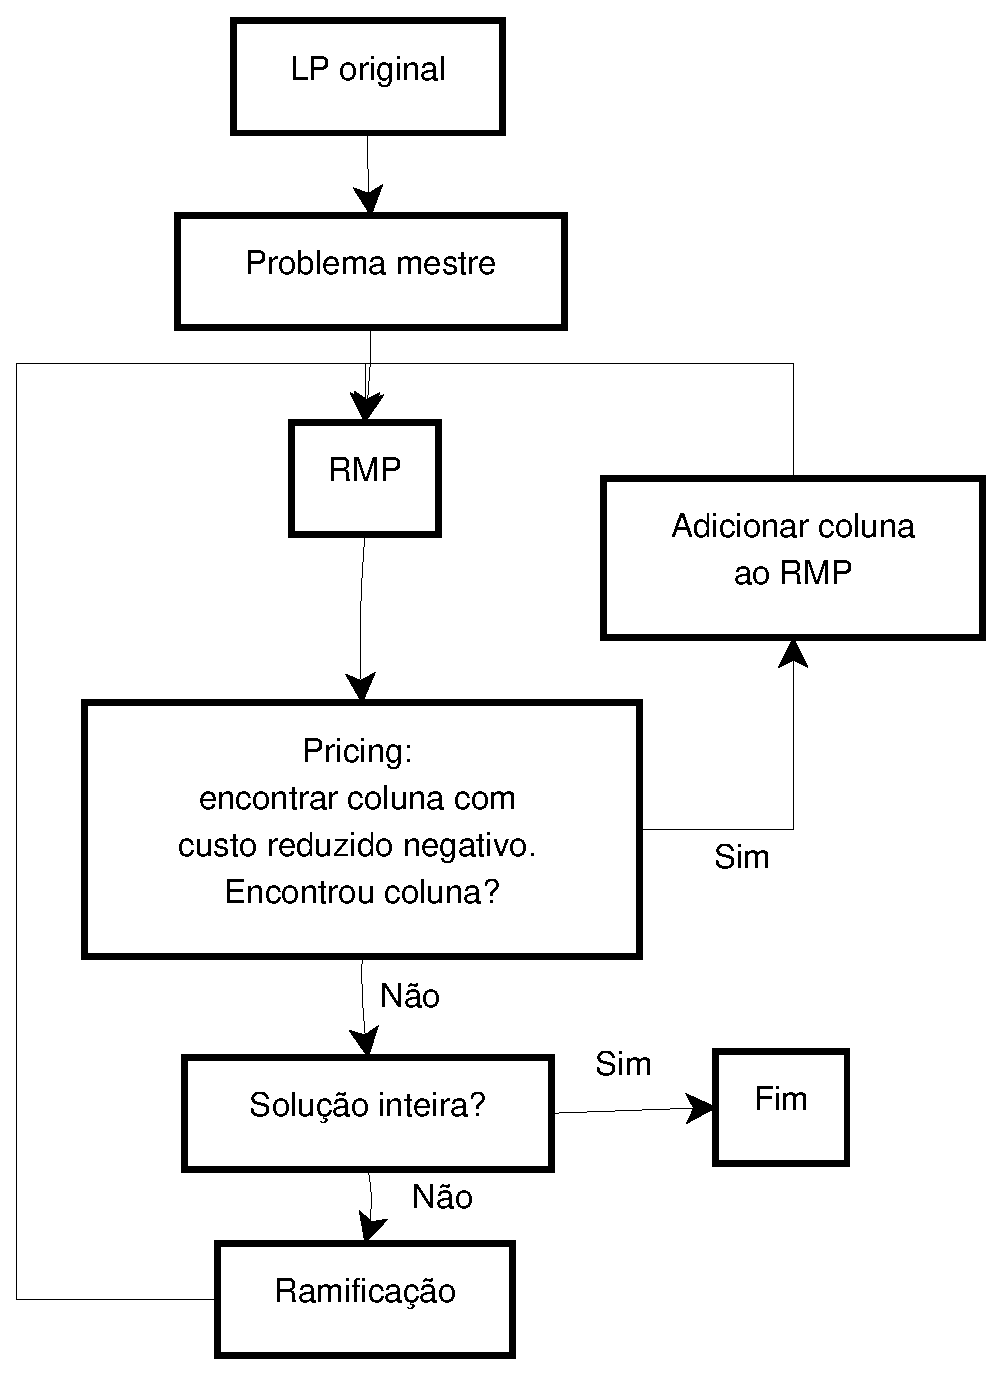
\includegraphics[scale=0.55]{figuras/branch_and_price} % era 0.35
  \caption{Diagrama de funcionamento do \emph{branch-and-price} para PL de minimização}
  \label{fig:branch_and_price}
\end{figure}

\subsubsection{Heurísticas}
No contexto dos problemas de otimização, as \emph{heurísticas} são
algoritmos para encontrar soluções boas mas não necessariamente ótimas,
de maneira rápida~\cite{NemhauserW1999}. No método de B\&B, as heurísitcas
são interessantes  não só para gerar uma solução incumbente inicial, antes
de iniciar o método de B\&B propriamente dito, mas também para melhorar
a solução incumbente ao longo da excução do
B\&B~\cite{NemhauserW1999,MorrisonJSS2016}.

Considerando um problema de otimização de minimização, uma heurística
\emph{primal} é aquela que gera uma solução viável do PL,
fornecendo uma cota superior para uma solução ótima.
Por outro lado, uma heurística \emph{dual} gera uma cota inferior para o PL.
%% Dentro do contexto de problemas de otimização, as \emph{heurísticas} são
%% algoritmos que não necessariamente retornam uma solução ótima. Como
%% abordado em \cite{NemhauserW1999}, elas são elaboradas para gerar soluções
%% boas 

Dentre as referências sobre otimização combinatória, mencionamos~\cite{Wolsey1998,BarnhartJNSV1998,NemhauserW1999,DesrosiersL2005,MorrisonJSS2016}.

\section{Algoritmos de aproximação}
Seja $\Pi = (E, w, \Scal)$ um POC, e seja $\Ical$ o seu conjunto de instâncias.  Para cada instância $I \in \Ical$, seja $\opt(I)$ o valor de uma solução ótima para a instância $I$.
%% e seja $sol(I)$ o conjunto de soluções viáveis de $I$.
%% Seja um POC $\Pi = (\Ical, E, w, \Scal)$.
Seja $A$ um algoritmo polinomial para $\Pi$ tal que, para cada instância $I \in \Ical$, $A(I)$ devolve uma solução viável de $I$.  Como dito no início da Seção \ref{sec:otimizacao}, para cada $S \in \Scal$, a função $f(S)$ devolve o valor associado à solução $S$.  Dizemos que o algoritmo $A$ é uma $\alpha$-aproximação para~$\Pi$,  problema de minimização, se, para toda instância $I \in \Ical$, temos que 
       $$f(A(I)) \leq  \alpha\,\opt(I).$$
Se $\Pi$ é de maximização, a desigualdade acima deve ser trocada por $\geq$.

% \begin{align*}
%   %% \label{afirm:same_arbs}
%   \alpha = \max\left(\frac{f(A(I))}{opt(I)}, \frac{opt(I)}{f(A(I)}\right).
% \end{align*}

O termo $\alpha$ (pode ser uma constante ou uma função de $I$) é
chamado \emph{fator de aproximação} do algoritmo $A$. 
Dizemos que um problema $\Pi$ de minimização tem um  \emph{fator de
  inaproximabilidade} $\beta$ se $\Pi$ não admite uma
$\alpha$-aproximação onde $\alpha\leq \beta$. 

%  Quando dizemos
% que um POC possui um \emph{limite de inaproximibilidade} $\beta$, significa que não existe uma $\alpha$-aproximação para o problema, onde $\alpha \leq \beta$ (respectivamente, $\alpha \geq \beta$), se o problema é de minimização (respectivamente, maximização).

Um algoritmo $A$ é um \emph{esquema de aproximação de tempo
  polinomial} (\emph{Polynomial-Time Approximation Scheme}), ou
simplesmente PTAS, para um problema  $\Pi$ de minimização se, para
cada instância de $\Pi$ e para cada racional \emph{fixo} $\epsilon >
0$, produz em tempo polinomial uma $(1 + \epsilon)$-aproximação.  Um
PTAS pode não ser muito útil do ponto de vista prático quando o
expoente do polinômio cresce muito à medida que o valor de $\epsilon$ diminui.  Uma variante deste esquema corresponde ao \emph{esquema
  eficiente de aproximação em tempo polinomial} (\emph{Efficient
  Polynomial-Time Approximation Scheme} - EPTAS), cujo tempo de
execução deve ser  $O(n^c)$, onde $n$ é  o tamanho da instância e $c$ é uma
constante; mas neste caso, a constante da notação $O$ pode depender de~$\epsilon$.

Ao leitor interessado em mais conceitos e resultados sobre algoritmos de aproximação, recomendamos consultar Ausiello et al~\cite{AusielloPMGCK1999} e Williamson e Shmoys~\cite{WilliamsonS2011}. 

%% Maiores informações sobre geração de colunas podem ser encontradas em
%% \cite{BarnhartJNSV1998,DesrosiersL2005}.

%%% Local Variables:
%%% mode: latex
%%% coding: utf-8
%%% eval: (auto-fill-mode t)
%%% eval: (LaTeX-math-mode t)
%%% TeX-master: t
%%% End:
